\section{Effective Hamiltonian in the mean-field approximation}
Consider the long-wave contribution $\Xi_L$ to the GPF, Eq.~(\ref{Xi_L}). Let's calculate $\Xi_L$ in the approximation when all $\vb k_i=0$
\begin{equation}
	\Xi_L^{(1)} = \int \exp(\mu^*\rho_0 -\frac{d(0)}{2} \rho_0^2 - \frac{a_4}{4!N_B} \rho_0^4) {\rm d} \rho_0.
\end{equation}
Since, as previously learned, $d(0) \propto \langle N \rangle_0$ and $a_4 \propto \langle N \rangle_0^2$, it is convenient to perform the following substitution of variables $\rho = \langle N \rangle_0 \rho_0'$ in the the above expression and obtain
\begin{equation}
	\Xi_L^{(1)} = \langle N \rangle_0 \int \exp[\langle N \rangle_0 E(\rho'_0)] {\rm d} \rho'_0
\end{equation}
where the following notations were introduced
\begin{equation}
	E(\rho'_0) = \mu^*\rho_0' - \frac{d'(0)}{2} {\rho'}_0^2 - \frac{a'_4}{4!}{\rho'}_0^4,
\end{equation}
\begin{equation}
	d'(0) = \langle N \rangle_0 d(0) = a'_2 + \frac{6}{\pi}\eta \frac{\varepsilon}{k_BT} \frac{\hat{\Phi}_0}{\varepsilon\sigma^3}.
\end{equation}
\begin{equation}
	a'_2 = \langle N \rangle_0 a_2, \quad a'_4 = \frac{\langle N \rangle_0}{N_B} \langle N \rangle_0^2 a_4
\end{equation}
The presence of $\langle N \rangle_0$ in the exponent justifies the application of the steepest-descent method for integration. The result is the following
\begin{equation}
	\label{mf:Xi_L_1}
	\Xi_L^{(1)} = \langle N \rangle_0 \exp(\langle N \rangle_0 E(\rho_{0,{\rm max}}))
\end{equation}
where $\rho_{0,{\rm max}}$ maximizes the quantity $E(\rho'_0)$ and is found from the following conditions
\begin{equation}
	\frac{\partial E}{\partial \rho'_0} = 0; \quad \frac{\partial^2 E}{\partial {\rho'}_0^2} < 0.
\end{equation}
In explicit form these conditions become
\begin{equation}
	\label{eq_rho_mean_field}
	\mu^*-d'(0)\rho_0 - \frac{a'_4}{3!}{\rho'}_0^3 = 0,
\end{equation}
\begin{equation}
	-d'(0) - \frac{a'_4}{2}{\rho'}_0^2 < 0.
\end{equation}

\subsection{Naive approximation}
In the most simple approximation, the quantity $\mu^*$ plays the same role as an external magnetic field in the Ising model. For Ising model it is known that the critical point appears at the absence of the external field, thus to find the critical point in our approximation, one condition is 
$$\mu^*=0.$$ 
The quantity $\mu^*$ depends on the chemical potential, through the term $\beta(\mu - \mu_0)$, on the temperature, through the term proportional to $\alpha(0)$, and on the packing fraction $\eta.$
If we assume that $\mu = \mu_0$, then the condition $\mu^*=0$ will relate the temperature and $\eta$
$$
{\frak M_3}/{\frak M_4} + \alpha(0)\tilde{\frak M}_1 = 0.
$$


This is the first condition that relates these two quantities.
The second condition is obtained from the requirement that non-zero solution exists for $\rho'_0$:
$$ {\rho'}^3_0 + \frac{3!d'(0)}{a'_4}{\rho'}_0 = 0 $$

$$
\rho_{01} = 0;
$$ 

$$
\rho_{02,03} = \pm\sqrt{-\frac{3!d'(0)}{a'_4}}
$$

Since $a'_4$ is always positive in the region $0.04 \leq \eta \leq 0.22$, the solutions $\rho_{02}$ and $\rho_{03}$ are real when $d'(0) \leq 0$. Thus the second condition for the critical point is 
$$
d'(0) = 0
$$

Thus in explicit form the system of two equations relating the temperature and packing fraction is as follows
\begin{eqnarray}
	&&\frac{\mathfrak{m}_3}{\mathfrak{m}_4} + \frac{6\eta}{\pi} \frac{1}{T^*} \frac{\hat{\Phi}_0}{\varepsilon\sigma^3}
	\left(1 - \frac{\mathfrak{m}_2\mathfrak{m}_3}{\mathfrak{m}_4} + \frac{\mathfrak{m}_3^3}{3\mathfrak{m}_4^2} \right) = 0;
	\nonumber\\
	&& a'_2 + \frac{6\eta}{\pi} \frac{1}{T^*} \frac{\hat{\Phi}_0}{\varepsilon\sigma^3} = 0,
\end{eqnarray}
where $T^* = k_BT/\varepsilon$ is the reduced temperature.
The equation for finding the critical value of $\eta$ is 
\begin{equation}
	\label{eq:critical_dens}
	\frac{\mathfrak{m}_3}{\mathfrak{m}_4} - a'_2
	\left(1 - \frac{\mathfrak{m}_2\mathfrak{m}_3}{\mathfrak{m}_4} + \frac{\mathfrak{m}_3^3}{3\mathfrak{m}_4^2} \right) = 0.
\end{equation}
\begin{figure}[htbp]
	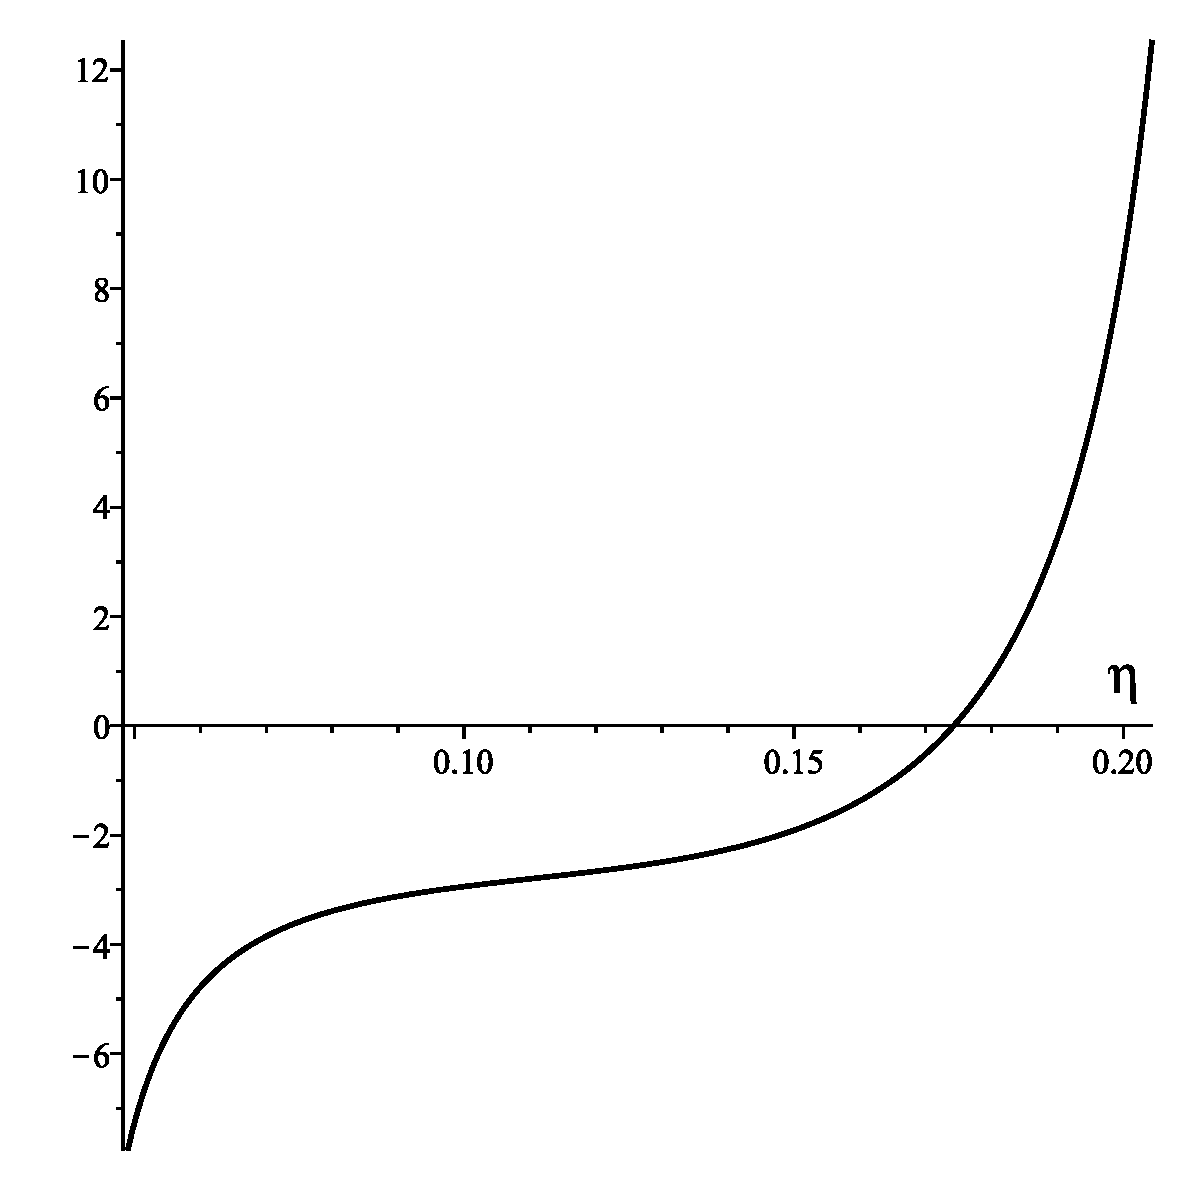
\includegraphics[width=0.7\textwidth,angle=0]{equation_for_critical_density}
	\caption{Equation~(\ref{eq:critical_dens}) for the critical packing fraction $\eta_c$.}
	\label{eq_for_eta_c}
\end{figure}
Figure~\ref{eq_for_eta_c} shows this equation graphically. The numerical solution to the equation gives the following value in the Percus-Yevick approximation
$$
\eta_c = 0.1742,
$$
or the critical value for the reduced density $\rho^* = \sigma^3\langle N \rangle / V$
$$
\rho^*_c = 0.3327.
$$
In the Carnahan-Starling approximation the corresponding values are
\begin{equation}
	\eta_c = 0.1766, \quad \rho^*_c = 0.3374.
\end{equation}
The critical temperature is now found
$$
T^*_c = -\frac{6\eta_c}{\pi a'_2} \frac{\hat{\Phi}_0}{\varepsilon\sigma^3}
$$
which for the parameters value $R_0/\alpha = 3.5$ is $T^*_c=2.14$ in Percus-Yevick approximation, and $T^*_c=2.15$ in the Carnahan-Starling one.
It is very important to note that both critical density and critical temperature depend on the parameters of the attractive part of potential. In particular, the critical temperature $T_c$ approaches zero as the interaction potential becomes more and more narrow ($\alpha \to \infty,$ $\hat{\Phi}_0 \to 0$).

The solutions to the equation~(\ref{eq_rho_mean_field}) for $\rho'_0$ can be written in general form via the discriminant of this cubic equation (via the Cardano's formulas). We are not going to do so for this simple approximation, but are going to integrate expression~(\ref{Xi_L}) over non-zero values of $k$, obtain similar equation for $\rho_0$ but with re-normalized coefficients, and investigate the obtained equation more closely.

\subsection{Applying condition $\langle N \rangle_0 = \langle N \rangle$}
Another way to address the problem of finding the critical point coordinates is to impose the condition of equality between particle numbers averages for the reference system and the whole system
\begin{equation}
	\langle N \rangle_0 = \langle N \rangle.
\end{equation}
This condition was, for example, applied in~\cite{YukhJSP1995}.

The general equation to find the average (equilibrium) number of particles is
\begin{equation}
	\left(\frac{\partial \ln\Xi}{\partial (\beta\mu)}\right)_{T,V} = \langle N \rangle.
\end{equation}
In the expression~\ref{Xi_as_prod} for the grand partition function $\Xi$ only $\Xi_L$ depends on the chemical potential. Taking into account its expression~\ref{Xi_L}, as well as the expression~\ref{mf:Xi_L_1} for $\Xi_L^{(1)}$, we arrive at the equation
\begin{equation}
	\langle N \rangle_0
	\left(
	\mathfrak{m}_1 + \frac{\mathfrak{m}_2 \mathfrak{m}_3}{\abs{\mathfrak{m}_4}} + \frac{\mathfrak{m}_3^3}{3\mathfrak{m}_4^2}  + \rho_0^{\rm{max}}
	\right) 
	= \langle N \rangle.
\end{equation}
Applying the conditions $\langle N \rangle_0 = \langle N \rangle$ and $\mathfrak{m}_1 = 1$, we get
\begin{equation}
	\rho_0^{\rm{max}} = - \left(\frac{\mathfrak{m}_2 \mathfrak{m}_3}{\abs{\mathfrak{m}_4}} + \frac{\mathfrak{m}_3^3}{3\mathfrak{m}_4^2}\right).
\end{equation}
In a number of works, see e.g.~\cite{YukhJSP1995,Yukh2013,Yukh2014}, the right-hand side expression is considered as a distinct quantity and is denoted as $\Delta$
\begin{equation}
	\label{def:Delta}
	\Delta \equiv - \left(\frac{\mathfrak{m}_2 \mathfrak{m}_3}{\abs{\mathfrak{m}_4}} + \frac{\mathfrak{m}_3^3}{3\mathfrak{m}_4^2}\right).
\end{equation}

Thus there are three conditions to be met at the critical point. The first one, which follows from the requirements of Ising model symmetry, is
\begin{eqnarray}
	\mu^* = 0.
\end{eqnarray}
The second one is
\begin{equation}
	d'(0) = 0,
\end{equation}
and the third one, which follows from the requirement that $\rho_0^{\rm{max}} = 0$ at the critical point, is
\begin{equation}
	\Delta = 0.
\end{equation}
From the last condition we can immediately find the value of the critical density. Solving the equation $\Delta = 0$ numerically gives us 
\begin{equation}
	\eta_c = 0.12867, \quad \rho^*_c = 0.24574
\end{equation}
in the Percus-Yevick approximation, and
\begin{equation}
	\eta_c = 0.13044, \quad \rho^*_c = 0.24913
\end{equation}
in the Carnahan-Starling approximation.
It worth noting that the condition $\Delta = 0$ is equivalent to $\mathfrak{M}_3=0$, and consequently to $\mathfrak{m}_3 = 0.$

The equation for the critical temperature follows from the second condition
\begin{equation}
	\label{T_c_Delta}
	T^*_c = -\frac{6\eta_c}{\pi a'_2} \frac{\hat{\Phi}_0}{\varepsilon\sigma^3} = -\frac{\rho^*_c}{a'_2} \frac{\hat{\Phi}_0}{\varepsilon\sigma^3}.
\end{equation}
Its numerical values for the potential parameter $R_0/\alpha = 3.5$ are $T^*_c=2.197$ and $T^*_c=2.202$ in the Percus-Yevick and Carnahan-Starling approximations, respectively.

There are a few important conclusions regarding results based on the condition $\langle N \rangle_0 = \langle N \rangle$. First, the value of the critical density does not depend on the parameters of the attractive part of the potential. This consequence is very contradictory since the critical density is the same for any form of $\Phi(r)$ at $r\geq \sigma$, including very weak interactions. 
The value of $\eta_c$ does not depend on the approximation used for the grand partition function calculation, and its mean-field value obtained in this work is the same as the one obtained in~\cite{YukhJSP1995}.

Second, the critical temperature does depend on the parameters of interaction, and approaches zero as the range of interaction becomes shorter and shorter ($\alpha \to \infty,$ $\hat{\Phi}_0 \to 0$).

\begin{table}[h]
	\caption{Critical values of chemical potential for different parameters $R_0/\alpha$.}
	\begin{center}
		\begin{tabular}{|c|c|c|}
			%\begin{tabular}{cccccccccc}
			\hline
			$R_0/\alpha$ \quad & $\beta(\mu_c - \mu_0)$ \quad & $\beta\mu^{\rm{ex}}_c$ \quad \quad \\
			\hline
			2.0  & 2.6699 & 4.0342 \\
			2.5  & 2.6228 & 3.9872 \\
			3.0  & 2.5812 & 3.9456 \\
			3.5  & 2.5453 & 3.9097 \\
			4.0  & 2.5143 & 3.8787 \\
			4.5  & 2.4877 & 3.8520 \\
			5.0  & 2.4645 & 3.8289 \\
			5.5  & 2.4444 & 3.8088 \\
			6.0  & 2.4268 & 3.7911 \\
			\hline
		\end{tabular}
	\end{center}
	\label{tab:critical_chem_potential}
\end{table}

In this approach we can also find the value of the chemical potential at the critical point. From the condition $\mu^*=0$ and Eq.~(\ref{mu_star}) we get
$$
\beta(\mu_c - \mu_0) = -\mathfrak{M}_3/\mathfrak{M}_4 - \alpha(0)\tilde{\mathfrak{M}}_1 
= -\mathfrak{m}_3/\mathfrak{m}_4 - \frac{6\eta}{\pi} \frac{\varepsilon}{k_{\rm{B}}T} \frac{\hat{\Phi}_0}{\varepsilon\sigma^3} \tilde{\mathfrak{m}}_1
$$
where the following notation was introduced by the analogy with Eq.~(\ref{def:tilde_M_1})
\begin{equation}
	\tilde{\mathfrak{m}}_1 = \mathfrak{m}_1 -\frac{\mathfrak{m}_2 \mathfrak{m}_3}{\mathfrak{m}_4} + \frac{\mathfrak{m}_3^3}{3\mathfrak{m}_4^2},
\end{equation}
Since $\mathfrak{m}_3 = 0$ at the critical point, and $\mathfrak{m}_1 = 1$, we get
\begin{equation}
	\beta(\mu_c - \mu_0) = -\frac{\rho^*_c}{T^*_c} \frac{\hat{\Phi}_0}{\varepsilon\sigma^3} = a'_2.
\end{equation}
The numerical values of the chemical potential difference at the critical point are summarized in Table~\ref{tab:critical_chem_potential} for different interaction parameters.

The chemical potential of a system can be represented as a sum of ideal and excess parts
$$
\mu = \mu^{\rm{id}} + \mu^{\rm{ex}}.
$$
Thus the difference $\beta(\mu - \mu_0)$ is essentially the difference between excess chemical potentials. The excess chemical potential of a hard-sphere system in the Carnahan-Starling approximation is
\begin{equation}
	\beta\mu^{\rm{ex}}_0 = \frac{8\eta - 9\eta^2 + 3\eta^3}{(1-\eta)^3}.
\end{equation}
At the critical density $(\beta\mu^{\rm{ex}}_0)_c = 1.3644$. Thus, we can calculate the excess chemical potential of the whole system at the critical point. The results are presented in Table~\ref{tab:critical_chem_potential}.
